\documentclass[9pt,twocolumn,twoside]{opticajnl}
\journal{opticajournal}

\setboolean{shortarticle}{true}

\title{Chest X-Ray Pneumonia Classification using
CNN algorithm}

\author[1]{Naseim Ghribi}
\author[2]{Rasul Osmanbayli}
\author[3]{Omar Huseynov}

\affil[1]{naseimghribi@stu.aydin.edu.tr, Y2213.140001, Department of Computer Engineering, Aydin University, Istanbul, Turkiye, 34443}
\affil[2]{rasulosmanbayli@stu.aydin.edu.tr, Y2213.011013, Department of Computer Engineering, Aydin University, Istanbul, Turkiye, 34443}
\affil[3]{omarhuseynov@stu.aydin.edu.tr, Y2213.011009, Department of Computer Engineering, Aydin University, Istanbul, Turkiye, 34443}

\begin{abstract}
Chest X-ray images are an important tool for pneumonia detection, and deep learning can be used to extract relevant information from them. However, the effectiveness of deep learning models depends on exploratory data analysis (EDA), which can provide information about the dataset and help choose the right machine learning model. 

This article discusses the importance of EDA in pneumonia detection and other types of problems, and how it can be used to understand the dataset, correlate features with real outputs, identify potential challenges, and guide preprocessing and modelling efforts. EDA allows for rich and exhaustive data exploration, enabling researchers to gain hidden insights into the dataset. Through statistical analysis and visualization techniques, EDA can identify important features, patterns, and anomalies in chest X-ray images. This information can be used to choose the right machine learning model and determine the necessary preprocessing steps.

\end{abstract}

\setboolean{displaycopyright}{false}

\begin{document}

\maketitle

\section{Introduction}
Exploratory Data Analysis (EDA) plays an important role in identifying potential issues in a dataset of chest X-ray images used for pneumonia detection. Its main purpose is to uncover hidden patterns and trends and provide guidance to researchers in making informed decisions about preprocessing and modelling methods. Below is a clear explanation of how EDA effectively supports these complex processes:

\subsection{Anomaly Detection}

EDA helps detect anomalies in the dataset of chest X-ray images. These anomalies can include image errors, labelling mistakes, and inconsistencies in image acquisition. By visually inspecting the images and analyzing statistics like pixel intensity distributions or image metadata, researchers can identify irregularities that may affect the accuracy and reliability of deep learning models. By using EDA, researchers can find and fix these anomalies, ensuring the dataset's quality and integrity.

\subsection{Data Distribution and Imbalance}

EDA enables researchers to analyze the distribution of different classes in the dataset, specifically pneumonia-positive and pneumonia-negative cases. Imbalanced class distributions can lead to biased models with compromised performance. Through EDA, researchers can assess the class distribution and detect significant imbalances. This valuable insight helps make informed decisions about data augmentation techniques, sampling strategies, or model adjustments to effectively address the imbalance and ensure precise pneumonia detection models during training.

\subsection{Data Quality Assessment}

EDA plays a crucial role in evaluating the quality of chest X-ray images. It helps researchers identify and resolve potential issues such as low resolution, noise, or artifacts. By visualizing the images and analyzing quality indicators, researchers can make informed decisions about preprocessing steps, including image enhancement, denoising, or standardization. By conducting EDA, researchers ensure that the dataset used for model training consists of high-quality images, thereby enhancing the model's ability to accurately detect pneumonia.

\subsection{Pattern and Trend Identification}

EDA plays a vital role in unveiling inherent patterns and trends within the dataset of chest X-ray images. Through wide analysis of the images and application of statistical techniques, researchers can effectively identify radiological features correlated with pneumonia. Understanding these underlying patterns helps in selecting appropriate preprocessing techniques, such as cropping, resizing, or filtering, to enhance relevant features and optimize the model's performance.

\subsection{Modelling Technique Selection}

EDA provides valuable insights that assist researchers in choosing suitable modelling techniques for pneumonia detection. By understanding the dataset's characteristics and patterns discovered through EDA, researchers can make informed decisions about adopting appropriate deep learning architectures, like Convolutional Neural Networks (CNNs), and optimizing hyperparameters. EDA helps align the modelling techniques with the unique features of chest X-ray images, thus improving the accuracy of pneumonia detection.

\subsection{Dataset Overview}

The Kaggle Chest X-Ray Images (Pneumonia) dataset is well-known and extensively studied for advancing pneumonia detection using deep learning techniques. This dataset, available on the Kaggle and Mendeley platforms, consists of a diverse collection of chest X-ray images carefully annotated for pneumonia classification. It includes a large number of high-resolution chest X-ray images from various healthcare institutions and sources. The dataset covers both pediatric and adult patients, ensuring a comprehensive representation of pneumonia cases across different age groups. This diversity in patient demographics enriches the dataset and facilitates the development of robust and generalizable pneumonia detection models. Each chest X-ray image in the dataset is labelled as either pneumonia-positive or pneumonia-negative, enabling researchers to use supervised learning approaches for model training. The pneumonia-positive class includes images with viral or bacterial pneumonia. These images are critical examples for training models to accurately identify pneumonia-related patterns and abnormalities in X-ray scans. In total, the dataset contains 5856  JPEG X-ray images categorized into three classes: Viral Pneumonia (1493 images), Bacterial Pneumonia (2780 images) and Normal cases (1583 images).

Figure \ref{fig:healthy-lung-scans} shows normal lung scans without bacteria or viruses.

\begin{figure}[ht]
\centering
\fbox{2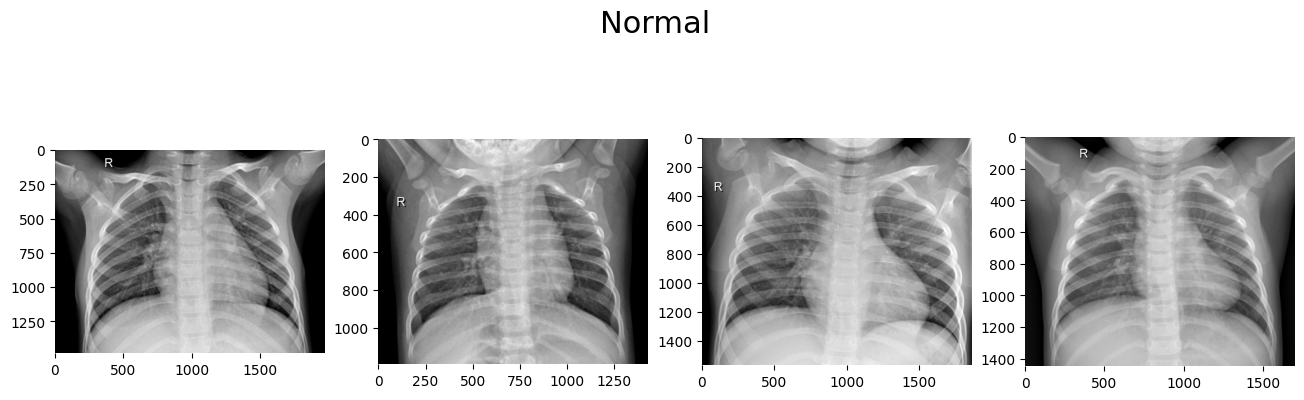
\includegraphics[width=\linewidth]{Images/normal_images.png}}
\caption{Healthy lung scans}
\label{fig:healthy-lung-scans}
\end{figure}

Figure \ref{fig:bacteria-lung-scans} shows the scans of lungs with a bacterial infection.

\begin{figure}[ht]
\centering
\fbox{2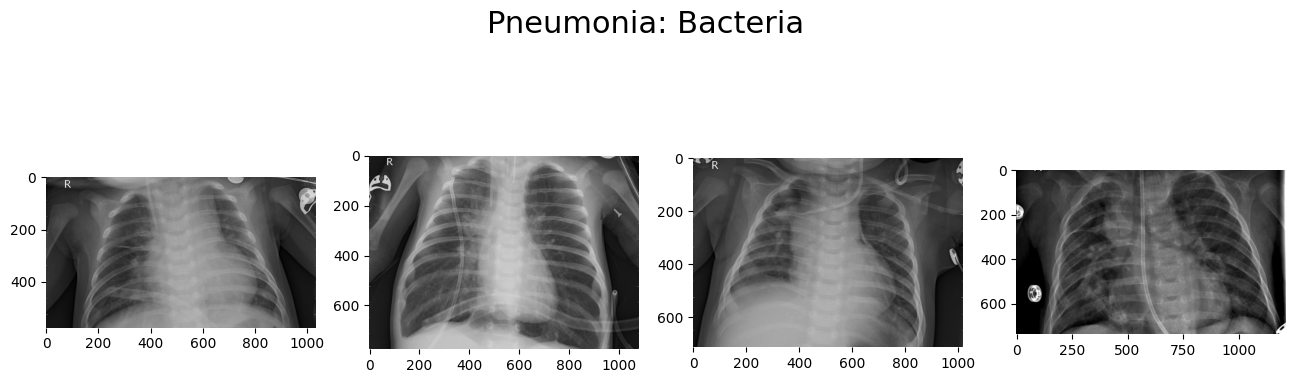
\includegraphics[width=\linewidth]{Images/bacteria_images.png}}
\caption{Lungs with bacterial infection}
\label{fig:bacteria-lung-scans}
\end{figure}

Figure \ref{fig:virus-lung-scans} shows the scans of lungs with viral infection.

\begin{figure}[ht]
\centering
\fbox{2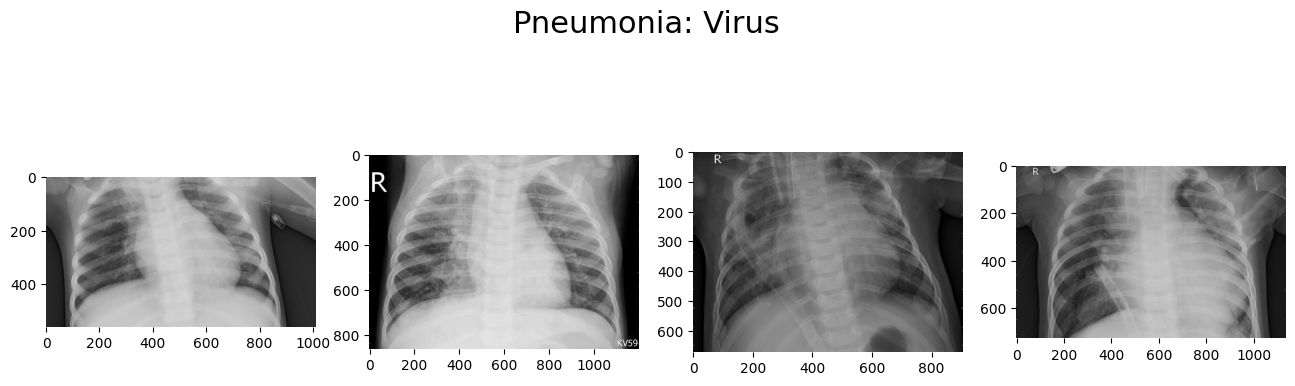
\includegraphics[width=\linewidth]{Images/virus_images.png}}
\caption{Lungs with viral infection}
\label{fig:virus-lung-scans}
\end{figure}

\section{Data Exploration}

Exploring the dataset is an important step in understanding the underlying patterns and trends in the data, which helps guide decisions about preprocessing and modelling. In this section, we will conduct an initial exploration of the dataset to gain insights into the distribution of data, class imbalances, and image characteristics.

To start, we can analyze how the pneumonia-positive and pneumonia-negative images are distributed in the dataset. Preliminary observations show a noticeable imbalance, with a significantly larger number of pneumonia-positive cases compared to pneumonia-negative cases. This imbalance poses challenges during model training because it may overly focus on the majority class, resulting in lower performance in pneumonia detection.

To address this issue, we can use various techniques like data augmentation, oversampling, or undersampling to mitigate the class imbalance problem.

Figure \ref{fig:dist-images} shows the distribution of each category in the dataset in the form of a pie chart.

\begin{figure}[ht]
\centering
\fbox{2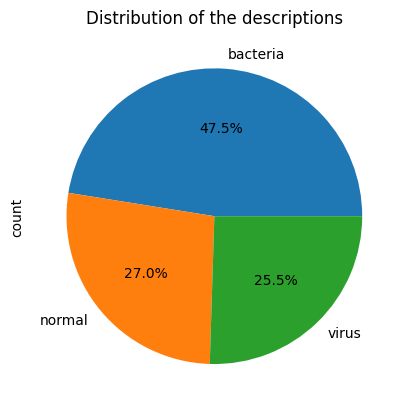
\includegraphics[width=\linewidth]{Images/dist_images.png}}
\caption{Distribution of the categories in the dataset}
\label{fig:dist-images}
\end{figure}

Figure \ref{fig:dist-images-bar-chart} shows the distribution of each category in the dataset in the form of a bar chart.

\begin{figure}[ht]
\centering
\fbox{2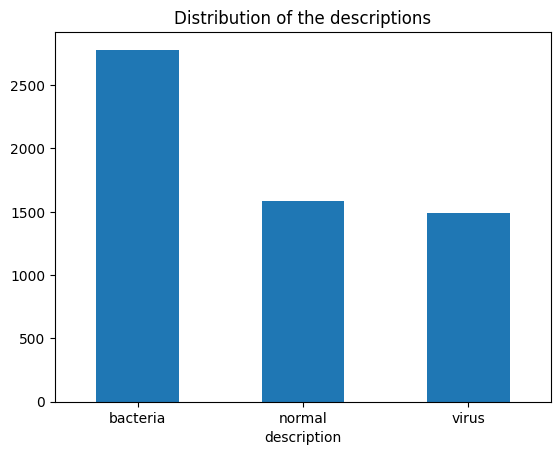
\includegraphics[width=\linewidth]{Images/dist_images_bar.png}}
\caption{Distribution of the categories in the dataset}
\label{fig:dist-images-bar-chart}
\end{figure}

Figure \ref{fig:normal-pixel-intensity} shows the average pixel intensity of healthy lungs.

\begin{figure}[ht]
\centering
\fbox{2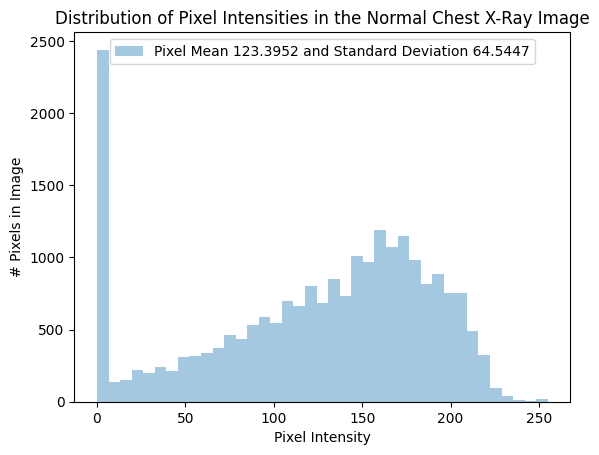
\includegraphics[width=\linewidth]{Images/normal_pixel_intensities.png}}
\caption{Average pixel intensity of healthy lungs}
\label{fig:normal-pixel-intensity}
\end{figure}

Figure \ref{fig:pneumonia-pixel-intensity} shows the average pixel intensity of lungs with pneumonia.

\begin{figure}[ht]
\centering
\fbox{2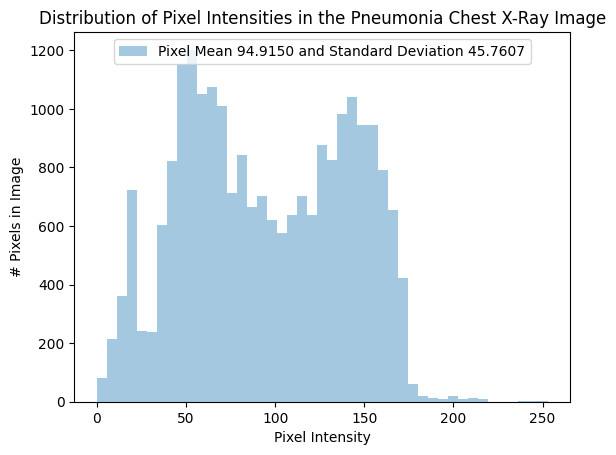
\includegraphics[width=\linewidth]{Images/pneumonia_pixel_intensities.png}}
\caption{Average pixel intensity of lungs afflicted with pneumonia}
\label{fig:pneumonia-pixel-intensity}
\end{figure}

Figure \ref{fig:pneumonia_and_normal_distribution} shows the pixel intensities in normal and pneumonia cases.

\begin{figure}[ht]
\centering
\fbox{2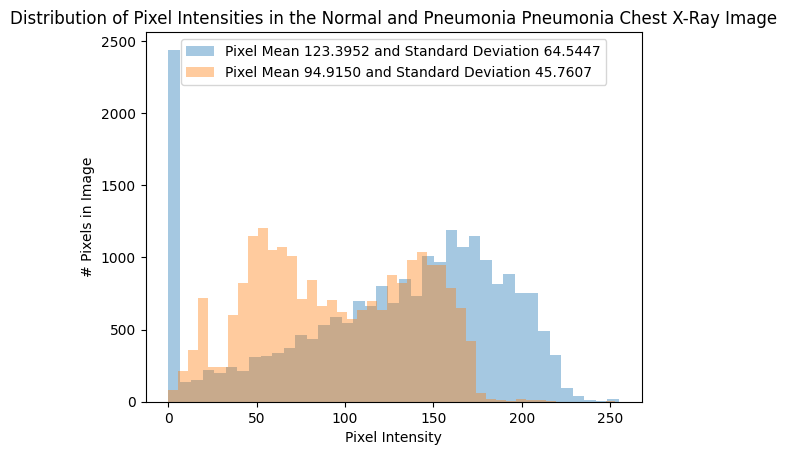
\includegraphics[width=\linewidth]{Images/pneumonia_and_normal_distribution.png}}
\caption{Pixel intensities in normal and pneumonia cases}
\label{fig:pneumonia_and_normal_distribution}
\end{figure}

\subsection{Image Augmentation}

Figure \ref{fig:differences_subplot} shows the differences between normal and pneumonia cases.

\begin{figure}[ht]
\centering
\fbox{2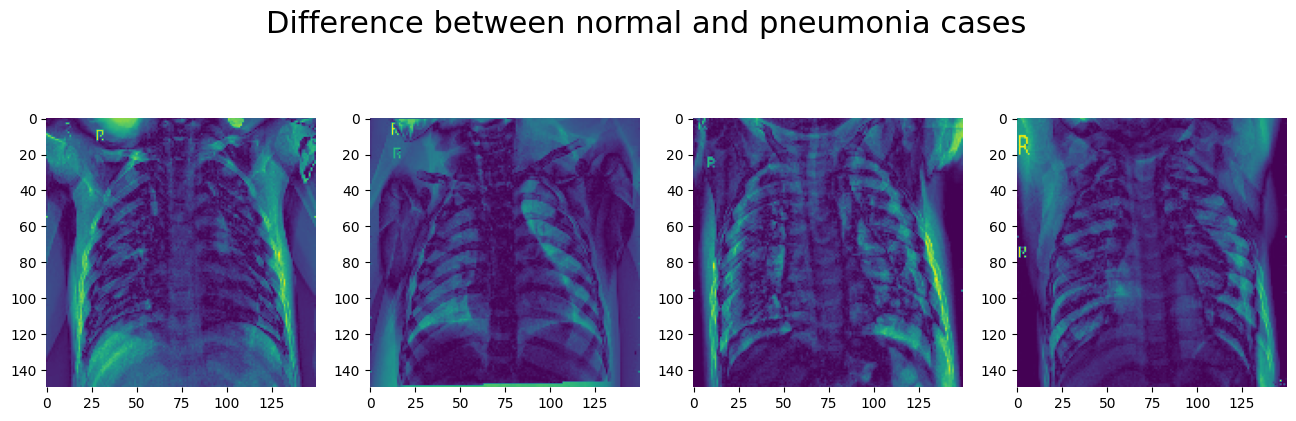
\includegraphics[width=\linewidth]{Images/differences_subplot.png}}
\caption{Difference between normal and pneumonia cases pixel by pixel}
\label{fig:differences_subplot}
\end{figure}

\subsection{Image Augmentation}

Data augmentation techniques are important for expanding the dataset and improving the model's ability to work with different examples. Since there are a limited number of pneumonia-positive cases, augmenting the data can help address the class imbalance problem and improve the model's ability to detect pneumonia. Augmentation techniques like rotation, flipping, zooming, and random cropping can be used to create additional variations of the existing images. However, it's crucial to make sure that the augmentations maintain the important characteristics and patterns related to pneumonia.


Figure \ref{fig:augmented-images} shows examples of augmented images from the dataset.

\begin{figure}[ht]
\centering
\fbox{2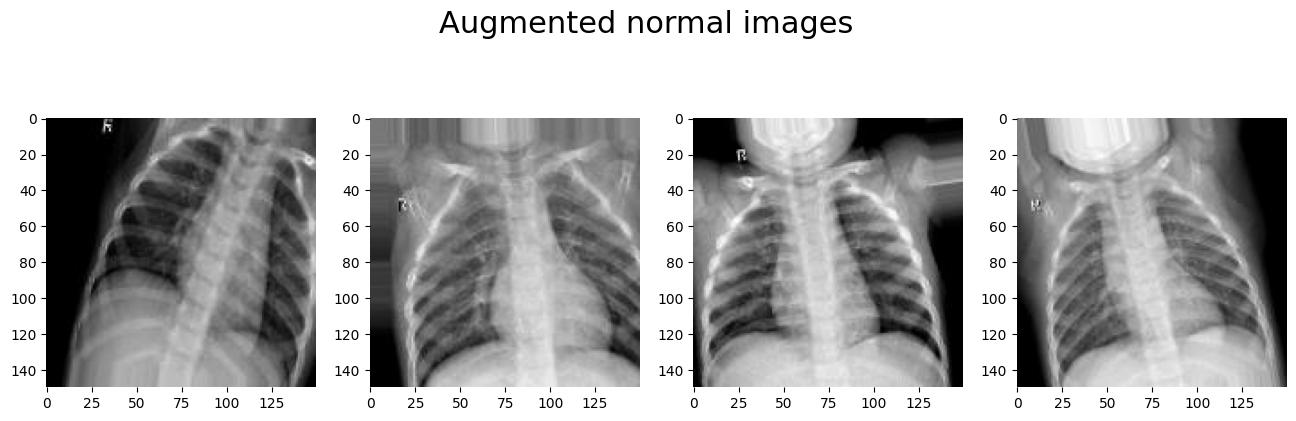
\includegraphics[width=\linewidth]{Images/augmented_images.png}}
\caption{Examples of augmented images}
\label{fig:augmented-images}
\end{figure}

\subsection{Handling Class Imbalance}

Data augmentation techniques play a pivotal role in expanding the dataset and enhancing the model's generalization capabilities. Considering the limited number of pneumonia-positive cases, data augmentation becomes particularly valuable in mitigating the class imbalance issue and improving the model's pneumonia detection proficiency. Techniques such as rotation, flipping, zooming, and random cropping can be applied to generate additional variations of the existing images. However, it is crucial to ensure that the augmentations preserve the essential characteristics and patterns associated with pneumonia, thereby retaining the informative content of the images.

\section{EDA Findings}

The EDA has revealed a significant class imbalance in the dataset, indicating a larger number of pneumonia-negative cases compared to pneumonia-positive cases. This emphasizes the need to address the class imbalance to prevent bias toward the majority class. Techniques like data augmentation, oversampling, or undersampling can be used to rebalance the classes and improve the model's performance in detecting pneumonia.


EDA analysis also revealed that the number of pneumonia-negative cases in our dataset was very limited, so we needed to use data augmentation techniques. We used techniques such as zooming images, applying shear functions, width and height shifting, and so on. We did not use techniques such as reflection because such images do not make sense in medical datasets. For example, after such a transformation, a person's heart would be on the right side. Pixel distribution charts and pixel differences between pneumonia positive and negative cases provided us with useful information about the correlation between some patterns on X-ray images and the presence of pneumonia in the patient's lungs.


In conclusion, the EDA findings offer crucial insights that guide subsequent steps in the pneumonia detection pipeline. Addressing class imbalance, applying image normalization techniques, considering patient characteristics, and ensuring data quality serve as guiding principles for pre-processing, modelling, and evaluation stages. By incorporating these findings into the subsequent steps, robust and accurate pneumonia detection models can be developed, taking into account the dataset's characteristics and enhancing diagnostic capabilities in clinical settings.


\begin{thebibliography}{9}
\bibitem{journal}
D. S. Kermany et al., “Identifying medical diagnoses and treatable diseases by image-based Deep Learning,” Cell, vol. 172, no. 5, 2018. doi:10.1016/j.cell.2018.02.010

\bibitem{journal}
X. Wang et al., “Chestx-Ray8: Hospital-scale chest X-ray database and benchmarks on weakly-supervised classification and localization of common thorax diseases,” 2017 IEEE Conference on Computer Vision and Pattern Recognition (CVPR), 2017. doi:10.1109/cvpr.2017.369

\bibitem{journal}
Shiraishi et al., “Development of a digital image database for chest radiographs with and without a lung nodule,” American Journal of Roentgenology, vol. 174, no. 1, pp. 71–74, 2000. doi:10.2214/ajr.174.1.1740071

\bibitem{journal}
H.-C. Shin et al., “Deep convolutional neural networks for computer-aided detection: CNN Architectures, dataset characteristics and transfer learning,” IEEE Transactions on Medical Imaging, vol. 35, no. 5, pp. 1285–1298, 2016. doi:10.1109/tmi.2016.2528162

\bibitem{journal}
P. Mooney, “Chest X-ray images (pneumonia),” Kaggle, https://www.kaggle.com/paultimothymooney/chest-xray-pneumonia (accessed May 17, 2023). 

\end{thebibliography}

\end{document}